\documentclass[11pt]{report}

\usepackage[a4paper,margin=2.7cm]{geometry}
\usepackage{graphicx}
\usepackage{booktabs}
\usepackage{amsmath}
\usepackage{hyperref}
\usepackage{xcolor}
\usepackage{caption}
\usepackage{parskip}
\usepackage{fancyhdr}
\usepackage{titlesec}

\hypersetup{colorlinks=true, linkcolor=blue!50!black, urlcolor=blue!50!black, citecolor=blue!50!black}
\captionsetup{font=small, labelfont=bf}
\titleformat{\chapter}[hang]{\normalfont\huge\bfseries}{\thechapter.}{1em}{}
\pagestyle{fancy}
\fancyhf{}
\fancyhead[L]{IMDC 2026 -- Backtesting \& Baseline/ML Modeling Report}
\fancyhead[R]{\thepage}
\renewcommand{\headrulewidth}{0.4pt}

\title{\textbf{Infodengue--Mosqlimate Dengue Challenge (IMDC) 2026\\[4pt]
\Large Backtesting Harness, Baseline and Machine-Learning Models:\\ Methodology and Results Report}}
\author{Mosqlimate IMDC 2026 Project}
\date{\today}

\begin{document}

\maketitle
\thispagestyle{empty}

\begin{abstract}
\noindent
This report documents the forecasting pipeline built after the data audit and EDA (see the companion \emph{Data Audit and Exploratory Data Analysis} report): a leakage-safe backtesting harness with a full probabilistic scoring stack (weighted interval score and its exact pinball-loss / CRPS decomposition), three statistical baselines, and a machine-learning model (LightGBM quantile regression with conformal calibration). All models are evaluated on the four official retrospective folds across the 26 mandatory Brazilian states. Headline findings: the machine-learning model achieves the best raw mean WIS (1309 vs.\ 1327 for the strongest baseline) and the best calibration, and is markedly the most robust model on the anomalous 2024 outlier season; however, under a scale-free per-unit relative-WIS metric the climatological baseline edges it (0.376 vs.\ 0.384), because raw mean WIS is dominated by the largest states and the outlier year where the ML model wins most decisively. No single model dominates across all four folds -- the ML model wins folds 1--2 and loses folds 3--4 -- which motivates the ensemble approach planned next. The pipeline is fully tested (36 automated tests) and reproducible end to end.
\end{abstract}

\tableofcontents

% ============================================================
\chapter{Scope and Recap}
% ============================================================

The companion data/EDA report established the dataset's structure and integrity, the four official backtest folds, a confirmed 15-week data-leakage trap, and the temporal/spatial/covariate structure of the dengue signal (including a historic 2024 outlier season roughly four times any other year). This report covers the next stage: turning that understanding into scored forecasts.

Three questions are answered here:
\begin{enumerate}
\item How are probabilistic forecasts scored, and is that scoring code correct? (Chapter~2)
\item How well do simple statistical baselines forecast the four folds? (Chapter~3)
\item Does a machine-learning model beat those baselines, and how robust is that conclusion? (Chapter~4)
\end{enumerate}

All work targets the mandatory challenge: weekly dengue forecasts at the state level for 26 states (Esp\'irito Santo excluded), with a median and 50/80/90/95\% prediction intervals for every week of each target season.

% ============================================================
\chapter{The Backtesting Harness and Scoring}
% ============================================================

\section{Weighted Interval Score}
Forecasts are scored with the weighted interval score (WIS), the standard metric of the CDC/ECDC forecasting hubs and -- as we verified by reading the installed \texttt{mosqlient} package source directly -- exactly the metric the Mosqlimate platform itself uses. For a central $(1-\alpha)$ prediction interval $[l,u]$ and observation $y$, the interval score is
\[
\mathrm{IS}_\alpha(l,u,y) = (u-l) + \tfrac{2}{\alpha}\max(0,l-y) + \tfrac{2}{\alpha}\max(0,y-u),
\]
and the WIS over the four required intervals ($\alpha_k \in \{0.5,0.2,0.1,0.05\}$) plus the median $m$ is
\[
\mathrm{WIS}(F,y) = \frac{1}{K+\tfrac12}\Big[\tfrac12\,|y-m| + \textstyle\sum_k \tfrac{\alpha_k}{2}\,\mathrm{IS}_{\alpha_k}(l_k,u_k,y)\Big], \quad K=4.
\]

\section{The CRPS/pinball identity and why it matters for correctness}
WIS is not merely \emph{analogous} to the continuous ranked probability score (CRPS) -- it is exactly the mean pinball loss over the nine required quantile levels, via the identity
\(
\mathrm{IS}_\alpha(l,u,y) = \tfrac{2}{\alpha}\big[\mathrm{PB}_{\alpha/2}(l,y) + \mathrm{PB}_{1-\alpha/2}(u,y)\big],
\)
where $\mathrm{PB}_\tau(q,y)=(y-q)(\tau-\mathbf 1\{y<q\})$. Our implementation is built on a single \texttt{pinball\_loss} primitive so that this CRPS-approximation property is structural rather than incidental. This identity is also a free correctness check: the WIS computed from the interval formula and from the pinball formula must agree exactly. During development this check caught a real bug -- an early implementation divided by the number of quantiles (9) instead of $K+\tfrac12$ (4.5), silently halving every score. The two formulations, plus an independently vendored reference implementation, now form three cross-validated assertions in the test suite.

\section{Testing}
The scoring stack is validated by a hand-computed toy example (WIS $=2.56$ for a fixed forecast/observation pair, confirmed three independent ways), property tests (WIS reduces to absolute error with zero-width intervals; a perfect forecast scores zero; the dispersion/over/under-prediction decomposition sums back to WIS), and a Monte-Carlo coverage test (forecasting from a known negative-binomial distribution recovers nominal coverage within $\pm 3$ percentage points over 5000 draws). The complete suite is 36 automated tests covering leakage guards, fold boundaries, scoring, and every model.

\section{Leakage safety by construction}
The harness -- never an individual model -- applies the cutoff filtering that keeps each fold honest, and asserts the absence of the 15-week gap-week leak on every training frame before any model sees it. This is the single most important design decision in the pipeline: no model can reintroduce the leakage trap because no model is trusted to do its own cutoff filtering.

% ============================================================
\chapter{Baseline Models}
% ============================================================

Three statistical baselines were implemented, in increasing sophistication:
\begin{itemize}
\item \textbf{Naive} -- last observed value carried forward, with uncertainty from the empirical distribution of historical $h$-step changes.
\item \textbf{Seasonal-naive} -- the median (robust to the 2024 outlier by construction) of the same epidemiological week across prior years.
\item \textbf{Climatological-quantile} -- direct empirical quantiles of historical case counts in a $\pm2$-week window around each target epiweek. This model requires zero fitting, so it also served as the harness's first client: any discrepancy against an independent WIS recomputation could only be a harness bug, not a modeling artifact.
\end{itemize}

The baselines behave exactly as the forecasting literature predicts (Table~\ref{tab:leaderboard}): each is progressively better than the last, with the climatological-quantile baseline the strongest -- a genuinely hard-to-beat reference, as is typical in epidemic forecasting.

% ============================================================
\chapter{Machine-Learning Model}
% ============================================================

\section{Design}
The ML model is a LightGBM quantile-regression forecaster (one gradient-boosted model per quantile level, nine total), trained directly for multi-horizon forecasting: a single pooled model across all 26 states and all horizons, with the horizon and the target epiweek supplied as explicit features. Because only four true forecast origins exist per fold, the model is trained on a \emph{synthetic-origin panel} -- every historical week from 2014 onward becomes a candidate forecast origin, each crossed with horizons 1--67, yielding hundreds of thousands of training rows while evaluation remains strictly the four official windows.

Features are engineered to be strictly leakage-safe and are anchored at the forecast origin: autoregressive lags and rolling statistics of log-incidence; a target-relative seasonal anchor (the most recent same-epiweek value observed at or before the origin); calendar harmonics; origin-anchored climate summaries and ocean-oscillation indices; and static per-state climate-zone composition. The model works internally in log-incidence space -- stabilizing the extreme cross-state scale differences and the 2024 outlier found in the EDA -- and converts predictions back to case counts for scoring.

\section{Calibrating the intervals}
Independent gradient-boosted quantile fits are well known to produce over-narrow intervals, and ours were no exception: raw, the 50\% interval covered only 25\% of outcomes. We corrected this with conformalized quantile regression (CQR), which uses a contiguous time-block holdout to widen each interval to its empirically-correct size. This restored calibration to near-nominal on the full state set (Table~\ref{tab:coverage}, Figure~\ref{fig:coverage}) at essentially no cost in WIS, and makes the model's uncertainty defensible for publication.

\section{Results}

\begin{table}[htbp]
\centering
\begin{tabular}{@{}lrrr@{}}
\toprule
\textbf{Model} & \textbf{Mean WIS} & \textbf{Relative WIS} & \textbf{Median AE} \\
& (raw) & (vs.\ naive) & \\
\midrule
LightGBM (CQR) & \textbf{1309} & 0.384 & \textbf{1711} \\
Climatological-quantile & 1327 & \textbf{0.376} & 1859 \\
Seasonal-naive & 1459 & 0.511 & 1856 \\
Naive & 1664 & 1.000 & 2218 \\
\bottomrule
\end{tabular}
\caption{Overall backtest performance, averaged across all four folds, 26 states, and all horizons. \emph{Mean WIS} is the raw average (dominated by large states and the outlier fold); \emph{relative WIS} is the scale-free pairwise metric that weights every state--fold--horizon equally. The two metrics disagree on the winner -- see \S\ref{sec:disagree}.}
\label{tab:leaderboard}
\end{table}

\begin{table}[htbp]
\centering
\begin{tabular}{@{}lrrrr@{}}
\toprule
\textbf{Model} & \textbf{50\%} & \textbf{80\%} & \textbf{90\%} & \textbf{95\%} \\
\midrule
LightGBM (CQR) & 48.5 & 79.6 & 88.5 & 92.7 \\
Climatological-quantile & 47.6 & 73.4 & 82.1 & 85.0 \\
Seasonal-naive & 44.9 & 79.9 & 88.2 & 92.5 \\
Naive & 40.2 & 72.1 & 80.5 & 85.9 \\
\midrule
\textit{Nominal (target)} & \textit{50} & \textit{80} & \textit{90} & \textit{95} \\
\bottomrule
\end{tabular}
\caption{Empirical interval coverage (\%). After CQR calibration the ML model is the best-calibrated across all four interval levels.}
\label{tab:coverage}
\end{table}

\begin{figure}[htbp]
\centering
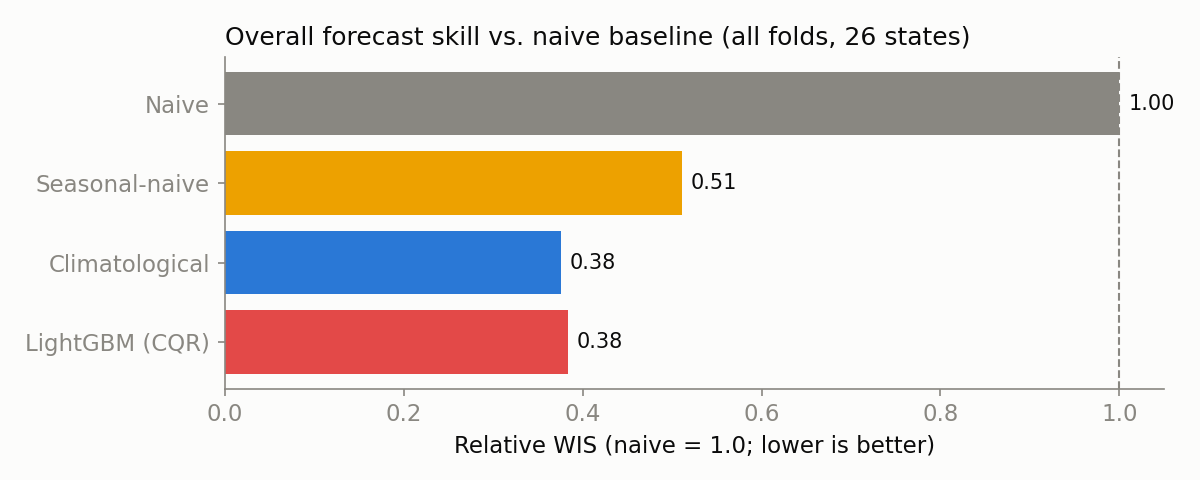
\includegraphics[width=0.85\textwidth]{../results/figures/model_relative_wis.png}
\caption{Overall forecast skill relative to the naive baseline (lower is better). On this scale-free metric the climatological baseline and the ML model are effectively tied, both roughly 62\% better than naive.}
\label{fig:relwis}
\end{figure}

\begin{figure}[htbp]
\centering
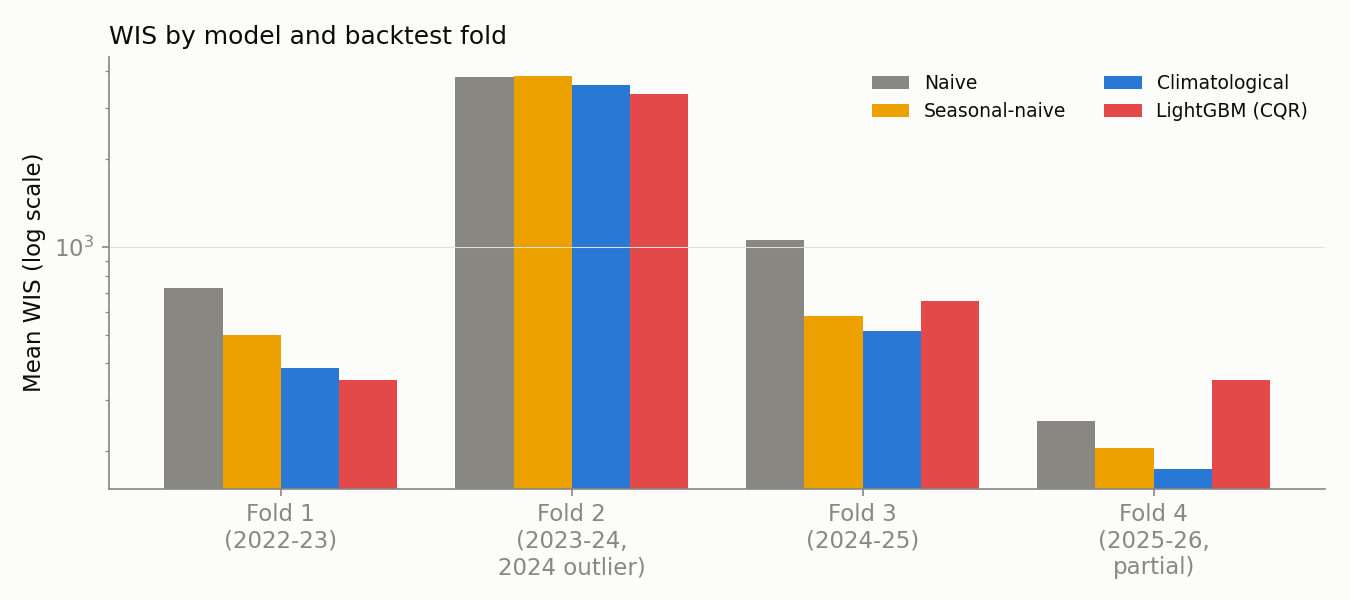
\includegraphics[width=0.95\textwidth]{../results/figures/model_wis_by_fold.png}
\caption{Mean WIS by model and fold (log scale). The 2024 outlier season (fold 2) is an order of magnitude harder than the others. The ML model wins folds 1 and 2 but loses folds 3 and 4; fold 4 is only partially resolved (data ends mid-season) and should be read cautiously.}
\label{fig:byfold}
\end{figure}

\begin{figure}[htbp]
\centering
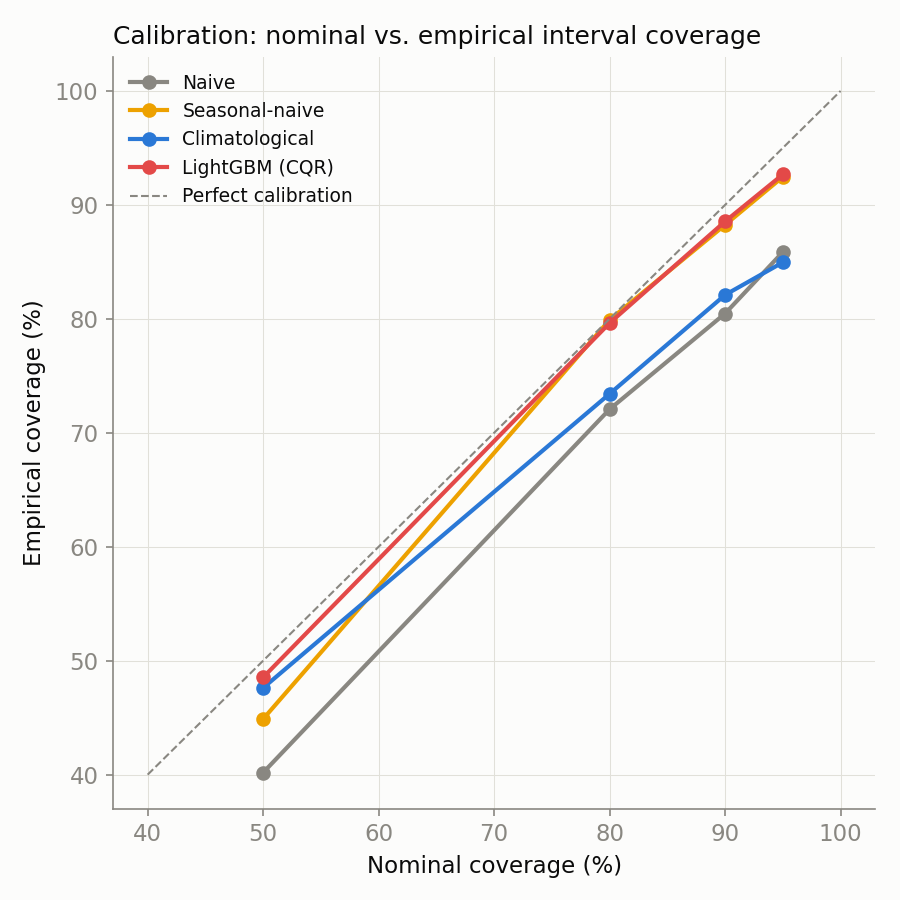
\includegraphics[width=0.62\textwidth]{../results/figures/model_coverage_diagram.png}
\caption{Calibration diagram: empirical vs.\ nominal interval coverage. Points on the dashed line are perfectly calibrated; the CQR-calibrated ML model tracks it most closely.}
\label{fig:coverage}
\end{figure}

\section{The two metrics disagree -- and that is the finding}
\label{sec:disagree}
The most important result in this report is not that one model ``wins,'' but that the answer depends on the aggregation, in a way that is itself informative. By raw mean WIS the ML model is best (Table~\ref{tab:leaderboard}, 1309 vs.\ 1327); by scale-free relative WIS the climatological baseline edges it (0.376 vs.\ 0.384; Figure~\ref{fig:relwis}). This is not a contradiction -- it is the direct consequence of the extreme cross-state skew documented in the EDA. Raw mean WIS is dominated by the largest states (S\~ao Paulo, Minas Gerais) and by the 2024 outlier fold, precisely where the ML model's superior point accuracy pays off most; the relative metric, which treats a small northern state's forecast as equal in weight to S\~ao Paulo's, rewards the climatological baseline's steadiness on the many smaller, noisier series. Both are legitimate; reporting only one would misrepresent the comparison. This scale-dependence was anticipated as a project risk and is why relative WIS is the primary cross-state metric going forward.

\section{No model dominates all folds}
Figure~\ref{fig:byfold} tells the second key story. The ML model wins fold 1 (351 vs.\ 386) and, most notably, the anomalous 2024 outlier fold 2 (3348 vs.\ 3588) -- exactly the season where robustness matters most for public-health preparedness. But it loses fold 3 (653 vs.\ 516), where it underpredicted the still-large 2025 season, and fold 4 (partial). A model that is best on average and most robust to the extreme season, yet not uniformly best, is the normal and honest outcome of a rigorous comparison -- and it is the empirical motivation for combining models rather than selecting one.

% ============================================================
\chapter{Summary and Next Steps}
% ============================================================

\section{What we have}
\begin{itemize}
\item A leakage-safe backtesting harness with a fully-tested WIS/CRPS/coverage scoring stack (36 automated tests, all passing), verified against the platform's own scorer.
\item Three statistical baselines and a calibrated machine-learning model, each scored across all four folds and 26 states, with reproducible per-unit results committed to \texttt{results/metrics/}.
\item A calibrated ML model that is the best-scoring model by raw WIS, the best-calibrated model, and the most robust model on the 2024 outlier season -- statistically tied with the climatological baseline on the scale-free metric.
\end{itemize}

\section{What this implies for the modeling to come}
The fold-by-fold split (Figure~\ref{fig:byfold}) is the clearest possible argument for an \emph{ensemble}: different models win different seasons, so a combination that is robust across seasons is likely to beat any single model on the metric that matters for a real forecast. The immediate next steps are therefore: (i) a deep-learning model (a small global recurrent network with a count-appropriate likelihood), (ii) a mechanistic/semi-mechanistic model grounded in per-season epidemic-curve fits, and (iii) an ensemble combining the strongest of all families, with weights tuned on a held-out fold distinct from those used for the headline comparison. The scale-free relative-WIS metric established here will remain the primary basis of comparison.

\section{Note on the validation-phase deadline}
The four backtest folds analysed here \emph{are} the challenge's validation-phase targets. The forecasts backing a validation submission therefore exist and are validated; what remains before an actual submission is packaging into the platform's exact file schema and uploading via the API (the latter requiring the team's API key). This is tracked as the packaging phase of the project.

\end{document}
